\documentclass[12pt]{article}

\usepackage{sbc-template}
\usepackage{graphicx,url}
\usepackage[utf8]{inputenc}
\usepackage[english]{babel}
\usepackage{tabularx}
\usepackage{booktabs}
\usepackage{multirow}
\usepackage{amsmath}
\usepackage{graphicx}
\usepackage{subcaption}
%\usepackage[latin1]{inputenc}  

     
\sloppy

\title{Federated learning for anomaly analysis in OBD-II sensor statistics and evaluation in edge devices}

\author{Renata Raffaine Villegas\inst{1}}


\address{Instituto de Computação -- Universidade Estadual de Campinas
  (UNICAMP)\\
  Caixa Postal 15.064 -- 13084-971 -- Campinas -- SP -- Brazil
  \email{r176635@dac.unicamp.br}
}

\begin{document} 

\maketitle

\begin{abstract}
This work investigates federated learning for anomaly detection in automotive OBD-II data using a normal-only autoencoder. Model performance is compared with local, centralized, and FedAvg training under IID data distributions, while FedAvg and FedProx are evaluated under non-IID distribution. The experimental setup has six clients, including five simulated on a computer and one running on a Raspberry Pi as a physical federated client. Beyond anomaly-detection performance, the study evaluates the computational and communication costs of the edge device participation, and shows how different local data volumes affect training time and resource utilization. A centralized supervised model is also included as a complementary reference. The results provide insights into the trade-offs between detection performance, data distribution, and computational constraints in federated automotive anomaly detection.

\end{abstract}
     

\section{intoduction}

The increasing availability of automotive sensor data creates opportunities for data-driven vehicle anomaly detection. However, centralized learning approaches require data from different vehicles to be collected in a common location, raising concerns regarding data privacy, communication overhead,
and scalability. Federated learning offers an alternative by enabling collaborative model training while keeping local data at each client.

The integration of Internet of Things (IoT) technologies has enabled the collection and analysis of massive amounts of data from on-board diagnostics (OBD-II) systems. However, the sheer volume of data and the heterogeneous nature of vehicular networks pose significant challenges for data processing and analysis. Federated Learning (FL) has emerged as a promising solution to address these challenges by enabling decentralized data analysis and model training without transferring raw data across devices. This work investigates the application of FL for anomaly detection in automotive OBD-II data using an unsupervised learning approach, specifically an autoencoder.

This work develops a model for anomaly detection using unsupervised learning and evaluates the performance of this model under both Independent and Identically Distributed (IID) and non-IID data distributions. We compare the performance of the federated learning models (FedAvg and FedProx) with local and centralized approaches. Additionally, we explore the deployment of these models on a Raspberry Pi, to evaluate the computational and communication costs.

The major contributions of this work are: providing insights into the trade-offs between performance, data distribution, and computational constraints in automotive FL. Specifically, we address the following questions:

1. Can federated learning achieve performance comparable to centralized training without transferring raw sensor data?

2. How do different data distributions (IID and non-IID) impact the performance and efficiency of federated learning models?

3. What are the computational and communication costs associated with training models on edge devices like the Raspberry Pi?

By addressing these questions, our study aims to provide a comprehensive evaluation of federated learning for anomaly detection in vehicular networks, highlighting its potential benefits and challenges.

\section{Related Work}

\section{Background}
\subsection{Automotive OBD-II Anomaly Detection}
\subsection{Unsupervised Learning and Autoencoders}
\subsection{Federated Learning}
\subsection{Federated Optimization under Data Heterogeneity}

\section{Experimental Setup}

This section presents the methodology and the experiments developed in this work. It presents the dataset and preprocessing procedures, the client data
partitioning strategy under IID and non-IID scenarios, the autoencoder architecture, and the supervised reference model. The major architecture of the federated learning system, the proposed experiments are also described. Finally, the evaluation metrics used to measure the anomaly detection performance and the computational and communication costs are introduced.


\subsection{Dataset and Preprocessing}

The dataset used in this work is available on Kaggle \cite{qasimghumman_obdii_dataset}. The dataset contains statistical features extracted from OBD-II sensor measurements collected from real and synthetic vehicles. It includes records from 39 real-vehicle sources as well as two synthetic data pools. Each sample represents a time window of vehicle operation, characterized by statistical descriptors of the monitored sensor signals. 

The dataset has labels to identify the origin of each record (real or synthetic) and to identify normal and abnormal values. Records from real vehicles are labeled as normal, whereas synthetic sources provide anomalous records and also some normal records. Additionally, the dataset contains additional information, including failure type, severity, and time-to-failure attributes. These variables were treated as metadata and excluded from the model inputs to prevent the models from relying on information directly associated with the failure labels or prediction targets. 



For the experiments, only sensor values were considered, so all contex-related and time-related labels were removed, leading to 105 available features, which corresponds to statistical descriptors —mean, standard deviation, maximum, minimum, and rate of change (ROC)—for each sensor signal. The source identifier and anomaly label were not used on the unsupervised learning trainings.

The data was normalized using a z-score scaler fitted using only the normal real-vehicle training samples. The resulting scaling parameters were applied across all clients and to the centralized, local, and federated models, including validation and test samples. Before model training, feature values were converted to 32-bit floating-point representation (float32), and non-finite values were imputed using the corresponding feature medians calculated from the training data.

It is important to notice that the dataset presents a strong association between the data source and the anomaly labels: real-vehicle records are normal, while the synthetic sources provide most of the anomalous examples. Therefore, the experiments evaluate anomaly detection using the available real and synthetic records, but do not establish the detection of faults observed in real vehicles. This limitation is considered when interpreting the experimental results.

\subsection{Data Partitioning}

For the centralized experiments, the dataset was divided into training, validation, and test sets, using target proportions of 70\%, 15\%, and 15\%, respectively. All records from a given real vehicle remained in the same partition. In contrast, the synthetic data pools were partitioned according to the anomaly label, since no vehicle or generation identifiers were available to identify the records.

For the Federated Learning experiments, the data was partioned to cover the  Independent and Identically Distributed (IID) and non-IID distribution. As the dataset does not give information about the real vehicles model and characteristics, the IID distribution was considered as the balanced distribution of normal real-vehicle training samples across the six clients. Table \ref{tab:IID-distribution} shows the data distribution on IID scenario.

\begin{table}[h!]
	\centering
	\label{tab:IID-distribution}
	\resizebox{\columnwidth}{!}{%
\begin{tabular}{|c|c|c|c|}
	\hline
	\textbf{Cliente} & \textbf{Vehicles in training} & \textbf{Training Samples} & \textbf{Test Samples}                 \\ \hline
	client\_1        & 5                             & 602                       & 178 normal / 178 anomally (356 total) \\ \hline
	client\_2        & 5                             & 765                       & 100 normal / 10 anommaly (200 total)  \\ \hline
	client\_3        & 5                             & 746                       & 168 normal / 168 anommaly (336 total) \\ \hline
	client\_4        & 4                             & 616                       & 190 normal / 190 anommaly (380 total) \\ \hline
	client\_5        & 4                             & 631                       & 137 normal / 137 anommaly (274 total) \\ \hline
	client\_6        & 4                             & 642                       & 157 normal / 157 anommaly (314 total) \\ \hline
\end{tabular}%
}
\end{table}

The non-IID scenario was designed to introduce differences in the amount of local training data available to each client. The data was splited using weights of ([1,1,2,2,4,4]), defining proportional targets of (1/14), (1/14), (2/14), (2/14), (4/14), and (4/14) of the total training samples for each client, respectively.  Table \ref{tab:non-IID-Distribution} shows the data distribution on non-IID scenario.

\begin{table}[h!]
	\centering
	\label{tab:non-IID-Distribution}
	\resizebox{\columnwidth}{!}{%
		\begin{tabular}{|c|c|c|c|c|}
			\hline
			\textbf{Client} & \textbf{Weigth} & \textbf{Vehicles in training} & \textbf{Trainig samples} & \textbf{Test Samples}                \\ \hline
			client\_1       & 1.0             & 2                             & 216                      & 165 normal / 165 anomaly (330 total) \\ \hline
			client\_2       & 1.0             & 2                             & 253                      & 120 normal / 120 anomaly (240 total) \\ \hline
			client\_3       & 2.0             & 4                             & 643                      & 130 normal / 130 anomaly (260 total) \\ \hline
			client\_4       & 2.0             & 4                             & 612                      & 159 normal / 159 anomaly (318 total) \\ \hline
			client\_5       & 4.0             & 6                             & 971                      & 365 normal / 365 anomaly (730 total) \\ \hline
			client\_6       & 4.0             & 6                             & 993                      & 351 normal / 351 anomaly (702 total) \\ \hline
		\end{tabular}%
	}
\end{table}

In both scenarios, records from the same real vehicle were kept together to preserve vehicle-level data integrity. First, complete vehicle groups were assigned to the six clients according to the corresponding allocation strategy. Then, each client's vehicle groups were divided into local training, validation, and test subsets. One vehicle per client was reserved for testing. For clients assigned at least four vehicles, one additional vehicle was reserved for validation, while the remaining vehicles were used for local training. 

Only samples belonging to the real vehicles were retained on training and validation data. Therefore, all synthetic records were excluded from both model optimization and early stopping, including synthetic records labeled as normal.  During early stopping, the reconstruction loss was calculated exclusively on normal real-vehicle validation samples, allowing model convergence to be assessed based on the reconstruction of normal operating conditions of real vehicles.

For the final anomaly detection evaluation, the complete test sets were used, retaining both real and synthetic records, including normal and anomalous samples. The reconstruction scores obtained for these samples were used to assess the ability of the autoencoder to distinguish normal from anomalous observations. The procedure for calibrating the anomaly detection threshold and the evaluation metrics are described in Section~\ref{subsec:evaluation_metrics}.

The supervised classifier was trained using all labeled training records, including normal and anomalous samples from real and synthetic sources. Its validation procedure also used the complete labeled validation set, while the final evaluation was performed on the complete test set. Therefore, the supervised classifier learned from both classes, whereas the autoencoder learned exclusively from normal real-vehicle records.

\subsection{Autoencoder Architecture}

The anomaly detection model is an undercomplete dense autoencoder designed to learn a representation of normal OBD-II sensor data. The input layer receives the 105 sensor-derived features described in Section~\ref{subsec:dataset_preprocessing}. The network  has a symmetric architecture with an encoder and a decoder with dimentions: \(105 \rightarrow 32 \rightarrow 8 \rightarrow 32 \rightarrow 105\). 

Rectified Linear Unit (ReLU) activation functions are used in the hidden layers, whereas the output layer uses a linear activation function to produce the reconstructed feature values. The resulting network has 7,409 trainable parameters.

The autoencoder is trained to minimize the mean squared reconstruction error between the input samples and their corresponding reconstructions. The Adam optimizer is used with a learning rate of 0.001 and a batch size of 32.

Training proceeds one epoch at a time, and the reconstruction loss is evaluated after each epoch using only normal real-vehicle validation samples. Whenever a lower validation loss is obtained, the corresponding model weights are saved. Training is terminated when the validation loss fails to improve according to the early-stopping criterion.

It was defined the maximum of 1,000 epochs, with an early-stopping patience of 50 epochs. For federated experiments, each client performs 5 local epochs per communication round, and the training process is limited to 200 communication rounds, with a patience of 10 rounds.


At inference time, the reconstruction error is used as an anomaly score: samples with larger reconstruction errors are considered more likely to deviate from the learned normal operating patterns. The classification threshold used to distinguish normal and anomalous samples is calibrated separately, as described in Section~\ref{subsec:evaluation_metrics}.


\subsection{Supervised Reference Model}

A supervised binary classifier was implemented as a reference model to provide a comparison with the autoencoder.  The classifier uses the same encoder topology as the autoencoder, which is $105 \rightarrow 32 \rightarrow 8 \rightarrow 1$.

The model is trained using the binary cross-entropy loss with logits. The Adam optimizer is used with a learning rate of 0.001 and a batch size of 32. Training is performed on a CPU.


The classifier is initialized with the pretrained weights of the autoencoder encoder and they are fine-tuned during supervised training. At inference time, sigmoid is applied to get the output. Samples with predicted probabilities greater than or equal to 0.5 are classified as anomalous, while the remaining samples are classified as normal.


\subsection{Federated Learning Architecture}

The federated learning architecture was implemented using the Flower framework and is described on  Fig \ref{fig:ArquiteturaGeral}. The SuperLink coordinates the execution, connects the nodes, and execute the agreggation. Each superNode hosts a client application identified by a unique client ID. 

\begin{figure}[h!]
	\centering
	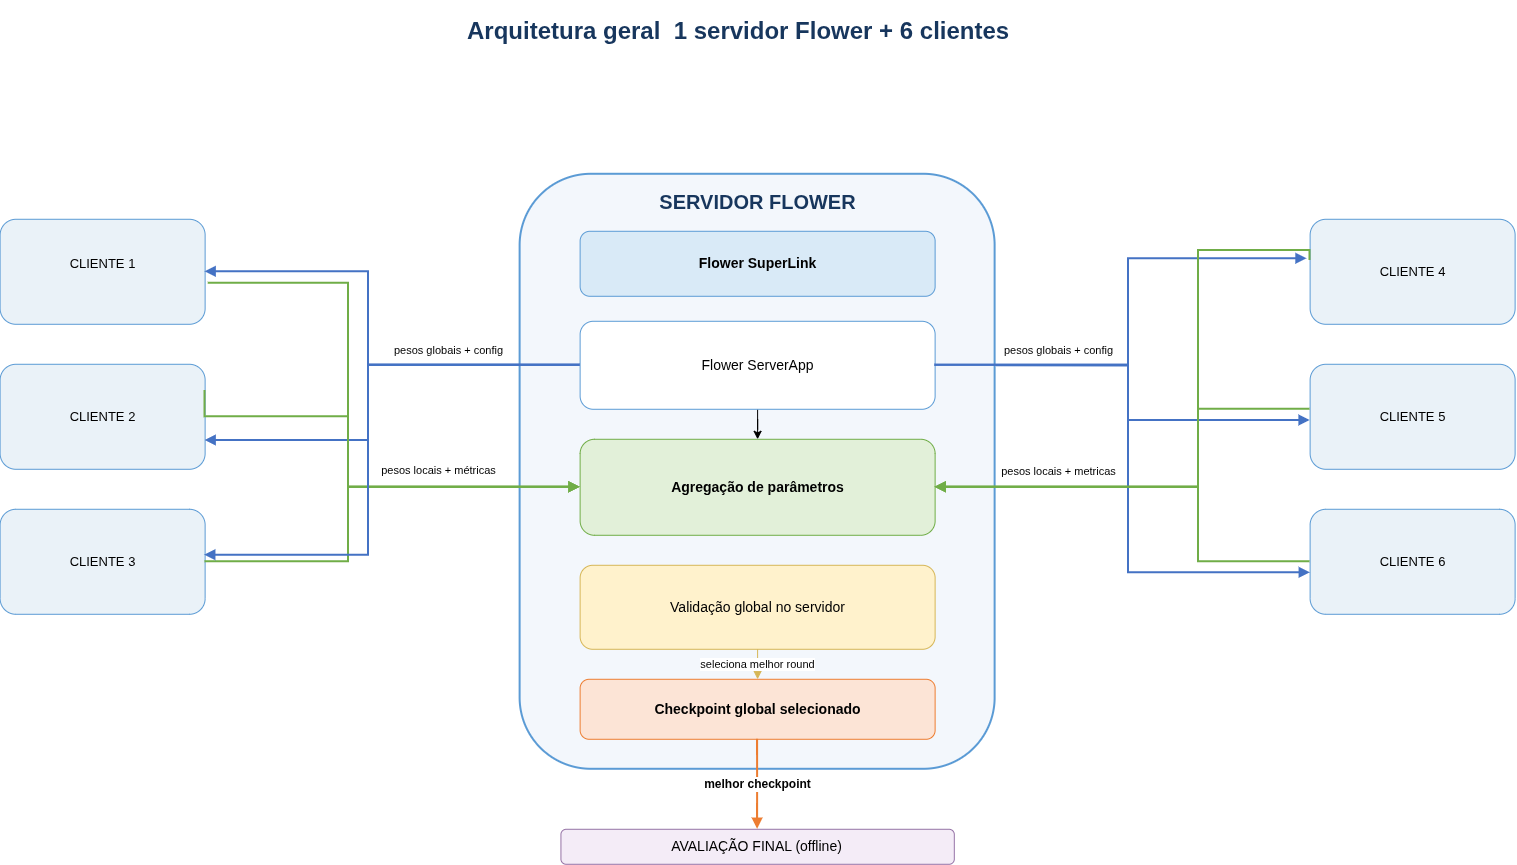
\includegraphics[width=.8\textwidth]{figures/Arquitetura geral.png}
	\caption{Federated Learning Architecture}
	\label{fig:ArquiteturaGeral}
\end{figure}


The experiments use six logical clients, each associated with a separate partition of the training data. All clients execute on the same host through separate Flower processes. The server initializes the global model parameters and coordinates the communication rounds according to the selected aggregation strategy, either Federated Averaging (FedAvg) or Federated Proximal (FedProx).

At the beginning of each communication round, the server distributes the current global model parameters and the round configuration to the participating clients. For this work, all clients participate of all rounds. Each client then performs five local training epochs using only its own normal samples collected from real vehicles. The same shared scaler is used on all clients, and raw training records remain local to each client. After local training, each client returns its updated model parameters and summary metrics, including the number of training examples, training loss, and training time.

The server aggregates the received model parameters using a weighted aggregation procedure based on the number of local training examples. Both FedAvg and FedProx use this aggregation rule, but FedProx uses a proximal regularization term to limit deviations from the global model parameters during local training.

After each aggregation round, the server checks the validation reconstruction loss and saves the weights whenever a lower validation loss is obtained. Training stops when the validation loss does not improve for 10 consecutive communication rounds or when the maximum of 200 rounds is reached. The best saved global checkpoint is subsequently evaluated offline using the test partition of each client.

Notice that the centralized validation is adopted to provide a common reference for global checkpoint selection across the experimental scenarios. This choice is particularly relevant to the quantity-skew partition, in which some clients do not have enough vehicle groups to form independent training, validation, and test subsets. Thus, the validation procedure does not depend on the availability of local validation groups at every client. During federated optimization, raw training records are not exchanged between clients and the server. 

\subsection{Hardware and Software Environment}

The experiments were conducted using a host machine and a Raspberry Pi 5 Model B. The host machine, which ran the Flower server and the simulated clients, was equipped with a 13th Gen Intel Core i5-13420H processor, featuring 8 physical cores and 12 logical processors, and 14 GiB of available system memory. The Raspberry Pi 5, used as a physical federated client, was equipped with a quad-core Cortex-A76 processor and 8 GB of RAM.

Both platforms used CPU-based model training. The host machine ran Ubuntu 26.04.1 LTS, while the Raspberry Pi ran Debian GNU/Linux 13 (Trixie). Python 3.14.4 was used on the host and Python 3.13.5 on the Raspberry Pi. Both environments used Flower 1.42.0 and PyTorch 2.14.1. Although the host environment used a CUDA-enabled PyTorch build, GPU acceleration was not used in the experiments; the Raspberry Pi used the CPU-only PyTorch build.

\subsection{Experimental Scenarios}
	

Four experimental configurations were considered to evaluate the autoencoder under different data distributions and client execution environments. The first two configurations use six simulated clients and compare centralized, local, and federated training methods. The IID scenario considers an approximately balanced allocation of training samples across clients, whereas the non-IID scenario uses different local data volumes to investigate the effects of client data heterogeneity.

The third and fourth configurations introduce a physical edge device into federated training. In these experiments, one of the six simulated clients is replaced by a Raspberry Pi 5, while the other five clients retain their original data partitions. Different clients are selected for replacement across experimental configurations to investigate the different local training-set sizes on the Raspberry Pi. FedAvg is evaluated in both configurations, while FedProx (($\mu=0.1$)) is additionally considered in the non-IID configuration.

Table~\ref{tab:experimental_scenarios} summarizes the experimental configurations and their respective objectives.


	\begin{table}[h!]
		\centering
		\caption{Experimental scenarios and evaluation objectives.}
		\label{tab:experimental_scenarios}
		\begin{tabularx}{\columnwidth}{|c|>{\hsize=0.9\hsize\raggedright\arraybackslash}X|>{\hsize=0.9\hsize\raggedright\arraybackslash}X|>{\hsize=1.2\hsize\raggedright\arraybackslash}X|}
			\toprule
			\textbf{Scenario}             & \textbf{Training methods}                       & \textbf{Client configuration}                                                                             & \textbf{Purpose}                                                                                \\ \midrule
			IID                           & Centralized, Local, FedAvg                      & Six simulated clients                                                                                     & Compare centralized, local, and federated learning under approximately balanced data distributions.         \\ \midrule
			Non-IID                       & Centralized, Local, FedAvg, FedProx ($\mu=0.1$) & Six simulated clients                                                                                     & Evaluate the effects of heterogeneous client data and compare FedAvg and FedProx.                           \\ \midrule
			IID                           & FedAvg                                          & Five simulated clients and one Raspberry Pi client, with different client assignments to the Raspberry Pi                                                      & Evaluate the participation of a physical edge device in federated training under IID conditions.           \\ \midrule
			\multicolumn{1}{|l|}{Non-IID} & FedAvg; FedProx ($\mu=0.1$)                     & Five simulated clients and one Raspberry Pi client, with different client assignments to the Raspberry Pi & Investigate how different local data volumes affect the computational cost of training on the Raspberry Pi. \\ \bottomrule
		\end{tabularx}
	\end{table}

\subsection{Evaluation Metrics}


The reconstruction error was used as the anomaly score, with higher values indicating a greater deviation from the learned normal operating patterns. A sample was classified as anomalous when its reconstruction error exceeded a predefined threshold ($\tau$). To calibrate this threshold without using labeled anomalous samples, the 95th and 99th percentiles of the reconstruction errors obtained from normal real-vehicle validation samples were considered. These configurations are referred to as the p95 and p99 thresholds, respectively. These thresholds were calibrated using the validation data and applied unchanged to the corresponding test sets.

The predicted class was compared with the ground-truth label, considering anomalous samples as the positive class. Accuracy, precision, recall, F1-score, and false positive rate (FPR) were used on evaluation. Accuracy measures the proportion of correctly classified samples, while precision describes the proportion of samples classified as anomalous that are actually anomalous. Recall measures the proportion of actual anomalies correctly identified by the model. The F1-score is the harmonic mean of precision and recall. The FPR quantifies the proportion of normal samples incorrectly classified as anomalous. These metrics were computed as follows:

\begin{align}
	\mathrm{Accuracy} &= \frac{TP+TN}{TP+TN+FP+FN} \\
	\mathrm{Precision} &= \frac{TP}{TP+FP} \\
	\mathrm{Recall} &= \frac{TP}{TP+FN} \\
	\mathrm{F1} &= 2 \cdot
	\frac{\mathrm{Precision}\cdot\mathrm{Recall}}
	{\mathrm{Precision}+\mathrm{Recall}} \\
	\mathrm{FPR} &= \frac{FP}{FP+TN}
\end{align}

where (TP), (TN), (FP), and (FN) are true positives, true negatives, false positives, and false negatives, respectively. These metrics were calculated for the $P-95$ and $P-99$ operating thresholds.

The Average Precision (AP) and the area under the Receiver Operating Characteristic curve (ROC-AUC) were also measured. AP calculates the weighted mean of precisions achieved at each recall threshold, with the weight corresponding to the incremental change in the recall. ROC-AUC measures the trade-off between the true positive rate and the false positive rate. The corresponding Precision-Recall and ROC curves were generated using the global test set.

For the Raspberry Pi experiments, computational performance was considered using local training time, average time per epoch, processing throughput, CPU utilization, peak memory consumption, and device temperature.

The throughput is calculated as the number of local training samples processed to the corresponding training time. These measurements were used to characterize the computational cost of executing local model updates on the physical edge device under different local data-volume conditions.


\section{Results}

\subsection{Six simulated clients}

\textbf{Six Simulated Clients}

This subsection presents the anomaly detection results obtained with six simulated clients under approximately balanced (IID) and quantity-skew data distributions. The centralized, local, and federated approaches are compared in terms of their detection performance. For the quantity-skew scenario, FedProx is additionally evaluated against FedAvg.

\textbf{Latent-Space Visualization}

Figure~\ref{fig:umap_latent} presents UMAP projections of the latent representations learned by the autoencoders for normal and anomalous test samples. The visualizations provide a qualitative analysis of how the different training approaches represent the two classes in the latent space.

\begin{figure*}[t]
	\centering
	\begin{subfigure}[b]{0.32\textwidth}
		\centering
		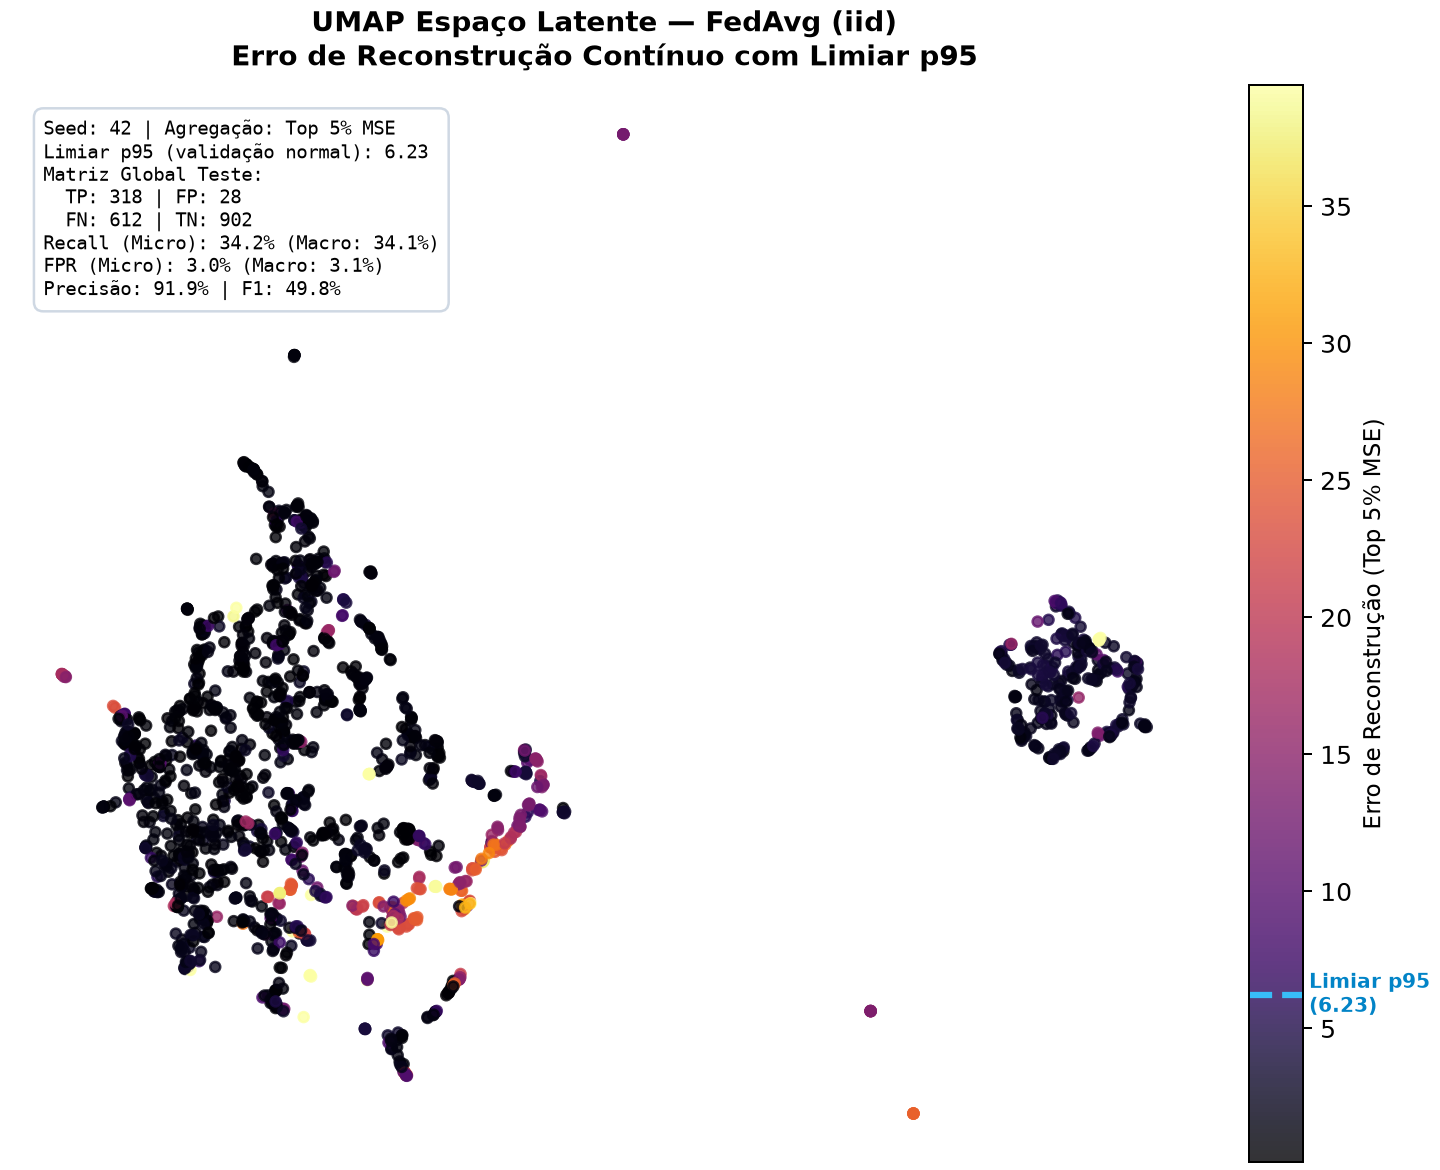
\includegraphics[width=\linewidth]{figures/fedavg_umap_errors_p95.png}
		\caption{FedAvg -- IID}
		\label{fig:umap_fedavg_iid}
	\end{subfigure}
	\hfill
	\begin{subfigure}[b]{0.32\textwidth}
		\centering
		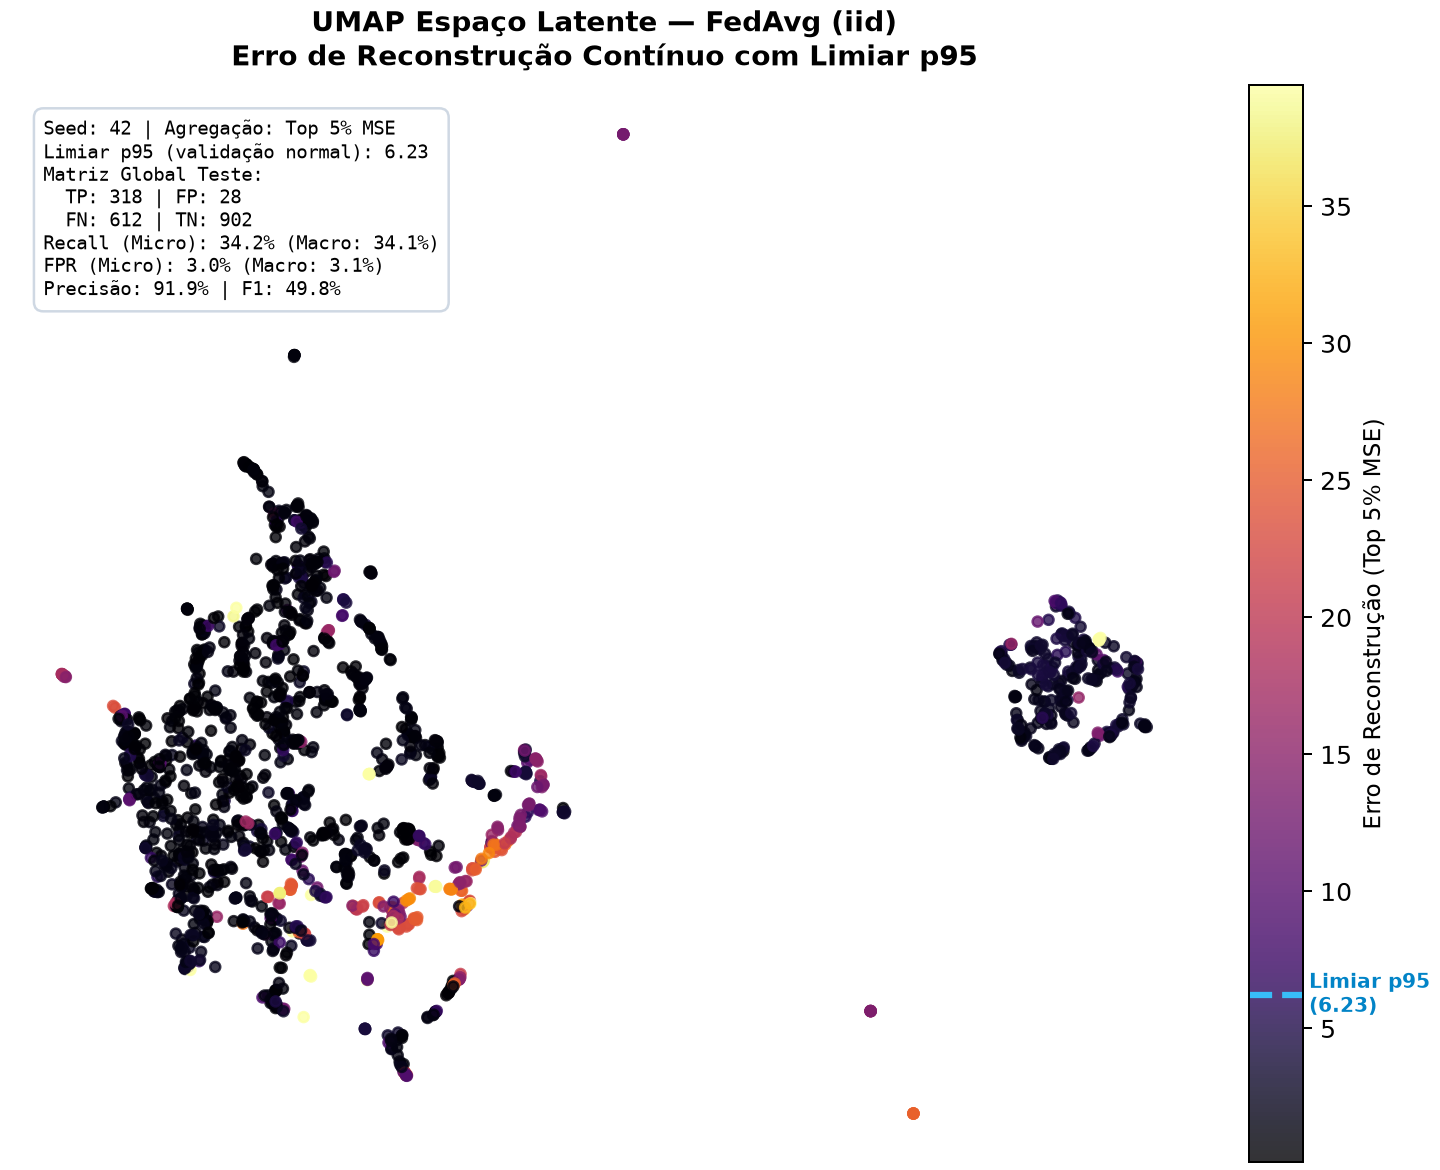
\includegraphics[width=\linewidth]{figures/fedavg_umap_errors_p95.png}
		\caption{FedAvg -- Quantity-skew}
		\label{fig:umap_fedavg_quantity}
	\end{subfigure}
	\hfill
	\begin{subfigure}[b]{0.32\textwidth}
		\centering
		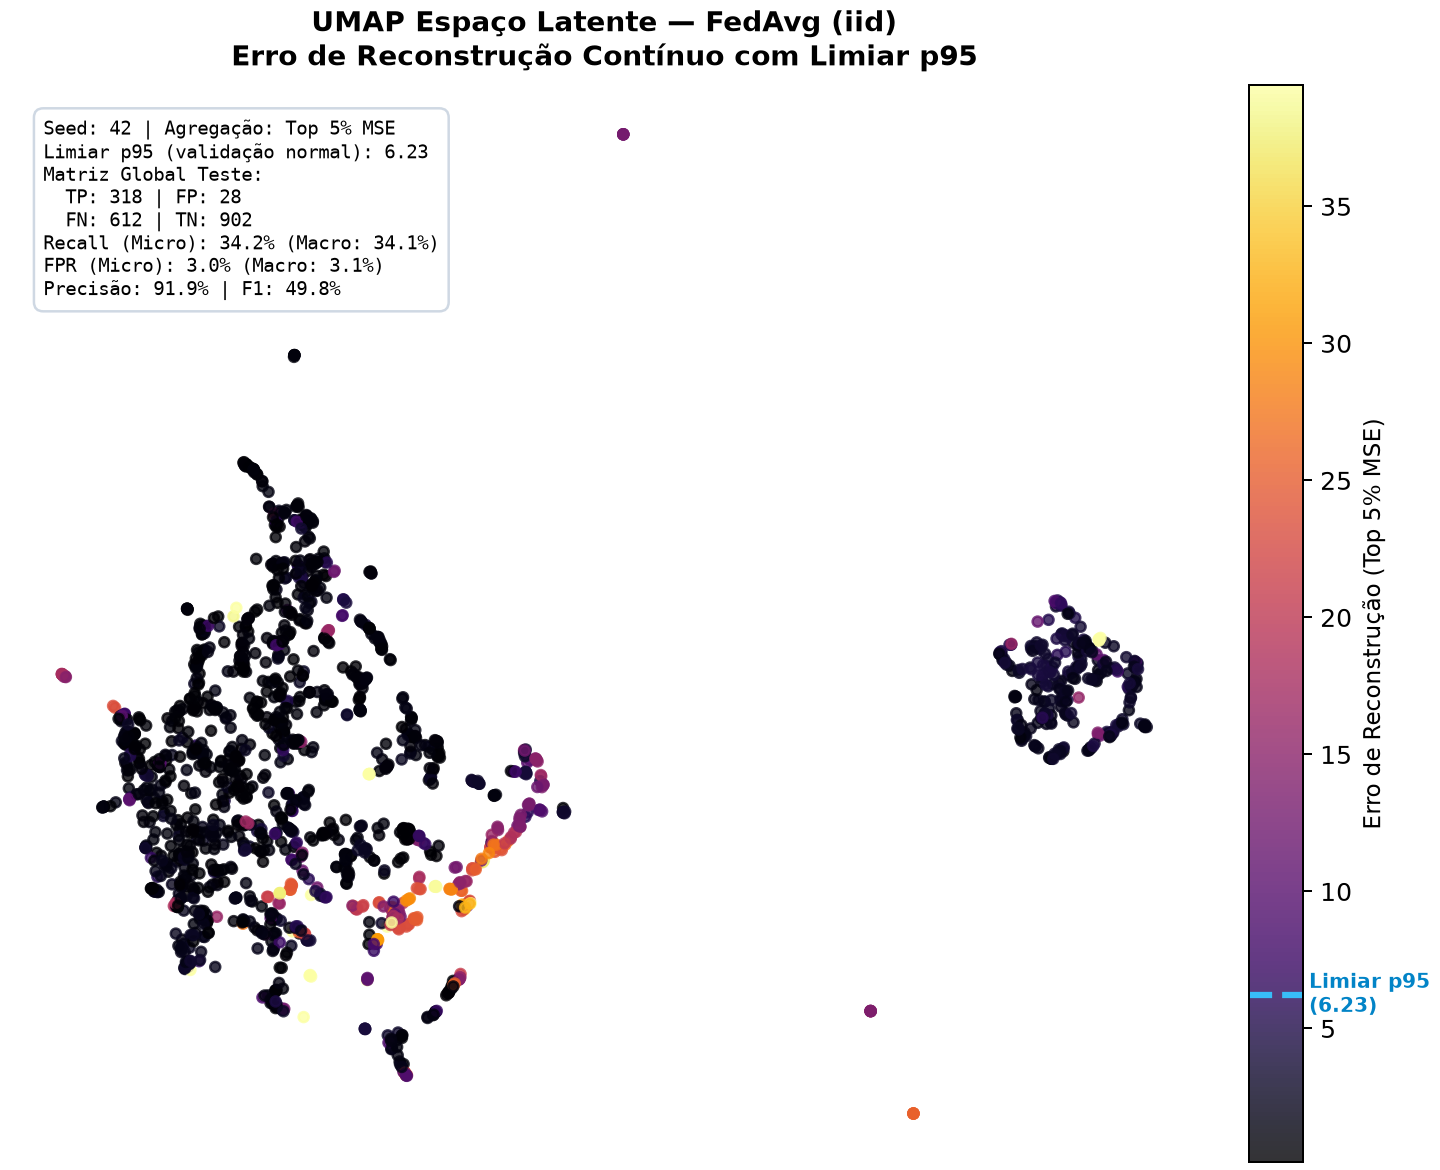
\includegraphics[width=\linewidth]{figures/fedavg_umap_errors_p95.png}
		\caption{FedProx -- Quantity-skew}
		\label{fig:umap_fedprox_quantity}
	\end{subfigure}
	\caption{UMAP projections of the autoencoder latent representations for normal and anomalous test samples under different federated learning configurations.}
	\label{fig:umap_latent}
\end{figure*}

\textbf{Detection Performance at Different Thresholds}

The detection performance was first evaluated using the P-95 threshold, calibrated from the reconstruction errors of normal real-vehicle validation samples. Table~\ref{tab:results_p95} reports the threshold-dependent metrics for the centralized, local, and federated approaches under both data distributions.

\begin{table*}[t]
	\centering
	\caption{Anomaly detection performance using the P-95 threshold. Values are reported as mean and standard deviation across experimental runs.}
	\label{tab:results_p95}
	\begin{tabular}{llccccc}
		\toprule
		\textbf{Scenario} & \textbf{Method} & \textbf{Accuracy} & \textbf{Precision} & \textbf{Recall} & \textbf{F1-score} & \textbf{FPR} \\
		\midrule
		IID & Centralized & $66.11 \pm 0.37$ & $91.43 \pm 0.50$ & $35.58 \pm 1.02$ & $51.19 \pm 1.00$ & -- \\
		IID & Local & $64.86 \pm 0.64$ & $92.14 \pm 0.49$ & $32.49 \pm 1.56$ & $47.99 \pm 1.64$ & -- \\
		IID & FedAvg & $57.87 \pm 0.28$ & $78.06 \pm 2.65$ & $20.31 \pm 0.34$ & $30.68 \pm 0.53$ & -- \\
		\midrule
		Quantity-skew & Centralized & $66.49 \pm 1.01$ & $84.19 \pm 2.19$ & $40.83 \pm 0.66$ & $54.88 \pm 1.13$ & -- \\
		Quantity-skew & Local & $59.01 \pm 1.10$ & $76.79 \pm 2.66$ & $37.79 \pm 1.14$ & $48.99 \pm 1.42$ & -- \\
		Quantity-skew & FedAvg & $55.23 \pm 0.17$ & $65.40 \pm 1.55$ & $24.65 \pm 0.10$ & $35.59 \pm 0.12$ & -- \\
		Quantity-skew & FedProx ($\mu=0.1$) & $59.58 \pm 0.44$ & $76.55 \pm 1.58$ & $37.33 \pm 0.97$ & $48.76 \pm 0.65$ & -- \\
		\bottomrule
	\end{tabular}
\end{table*}

Table~\ref{tab:results_p99} presents the results obtained using the P-99 threshold. This more conservative threshold allows the effect of a stricter anomaly decision criterion on the detection metrics to be examined.

\begin{table*}[t]
	\centering
	\caption{Anomaly detection performance using the P-99 threshold. Values are reported as mean and standard deviation across experimental runs.}
	\label{tab:results_p99}
	\begin{tabular}{llccccc}
		\toprule
		\textbf{Scenario} & \textbf{Method} & \textbf{Accuracy} & \textbf{Precision} & \textbf{Recall} & \textbf{F1-score} & \textbf{FPR} \\
		\midrule
		IID & Centralized & $57.86 \pm 1.04$ & $95.63 \pm 0.41$ & $16.51 \pm 2.17$ & $28.05 \pm 3.19$ & -- \\
		IID & Local & $56.41 \pm 0.37$ & $94.61 \pm 1.00$ & $13.62 \pm 0.81$ & $23.72 \pm 1.25$ & -- \\
		IID & FedAvg & $51.94 \pm 0.56$ & $79.66 \pm 3.05$ & $4.91 \pm 1.23$ & $9.07 \pm 2.11$ & -- \\
		\midrule
		Quantity-skew & Centralized & $57.68 \pm 0.95$ & $95.77 \pm 0.32$ & $16.08 \pm 1.99$ & $27.45 \pm 2.90$ & -- \\
		Quantity-skew & Local & $55.88 \pm 0.95$ & $92.94 \pm 3.12$ & $12.71 \pm 1.56$ & $22.33 \pm 2.51$ & -- \\
		Quantity-skew & FedAvg & $50.76 \pm 0.42$ & $55.52 \pm 1.44$ & $4.35 \pm 0.87$ & $7.92 \pm 1.48$ & -- \\
		Quantity-skew & FedProx ($\mu=0.1$) & $56.52 \pm 0.66$ & $93.86 \pm 1.37$ & $13.96 \pm 1.52$ & $24.24 \pm 2.27$ & -- \\
		\bottomrule
	\end{tabular}
\end{table*}

\textbf{Threshold-Independent Performance}

In addition to the threshold-dependent metrics, the models were evaluated using Average Precision (AP) and ROC-AUC, which are calculated from continuous anomaly scores. Unlike the previous metrics, these measures do not depend on the P-95 or P-99 decision thresholds.

Table~\ref{tab:results_threshold_independent} summarizes the threshold-independent results for each training approach and data distribution.

\begin{table}[t]
	\centering
	\caption{Threshold-independent anomaly detection performance.}
	\label{tab:results_threshold_independent}
	\begin{tabular}{llcc}
		\toprule
		\textbf{Scenario} & \textbf{Method} & \textbf{AP} & \textbf{ROC-AUC} \\
		\midrule
		IID & Centralized & -- & -- \\
		IID & Local & -- & -- \\
		IID & FedAvg & -- & -- \\
		\midrule
		Quantity-skew & Centralized & -- & -- \\
		Quantity-skew & Local & -- & -- \\
		Quantity-skew & FedAvg & -- & -- \\
		Quantity-skew & FedProx ($\mu=0.1$) & -- & -- \\
		\bottomrule
	\end{tabular}
\end{table}

\textbf{ROC and Precision-Recall Curves}

Figure~\ref{fig:global_curves} presents the ROC and Precision-Recall curves obtained from the global test set. These curves provide an additional comparison of the models across a range of decision thresholds, complementing the results reported in Tables~\ref{tab:results_p95} and~\ref{tab:results_p99}.

\begin{figure*}[t]
	\centering
	\begin{subfigure}[b]{0.48\textwidth}
		\centering
		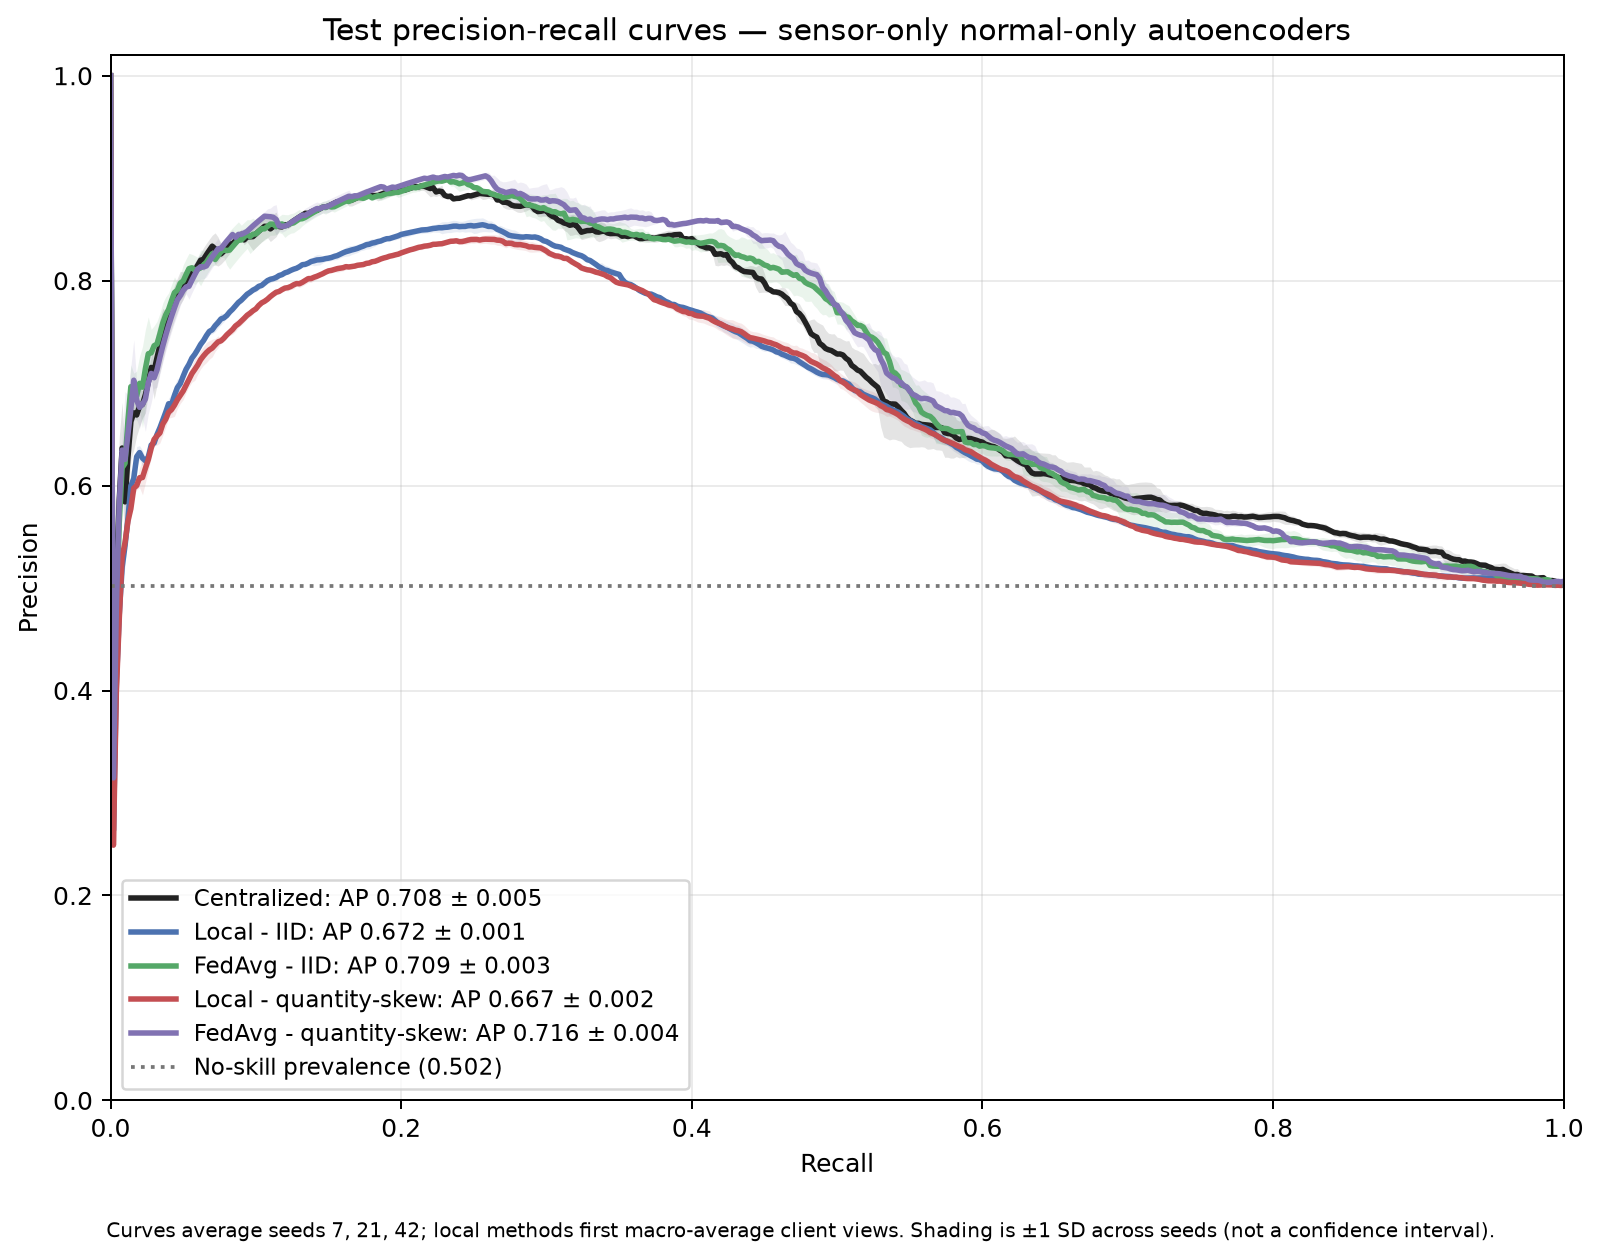
\includegraphics[width=\linewidth]{figures/precision_recall_test_sensor_only_seeds_7_21_42.png}
		\caption{ROC curves}
		\label{fig:global_roc}
	\end{subfigure}
	\hfill
	\begin{subfigure}[b]{0.48\textwidth}
		\centering
		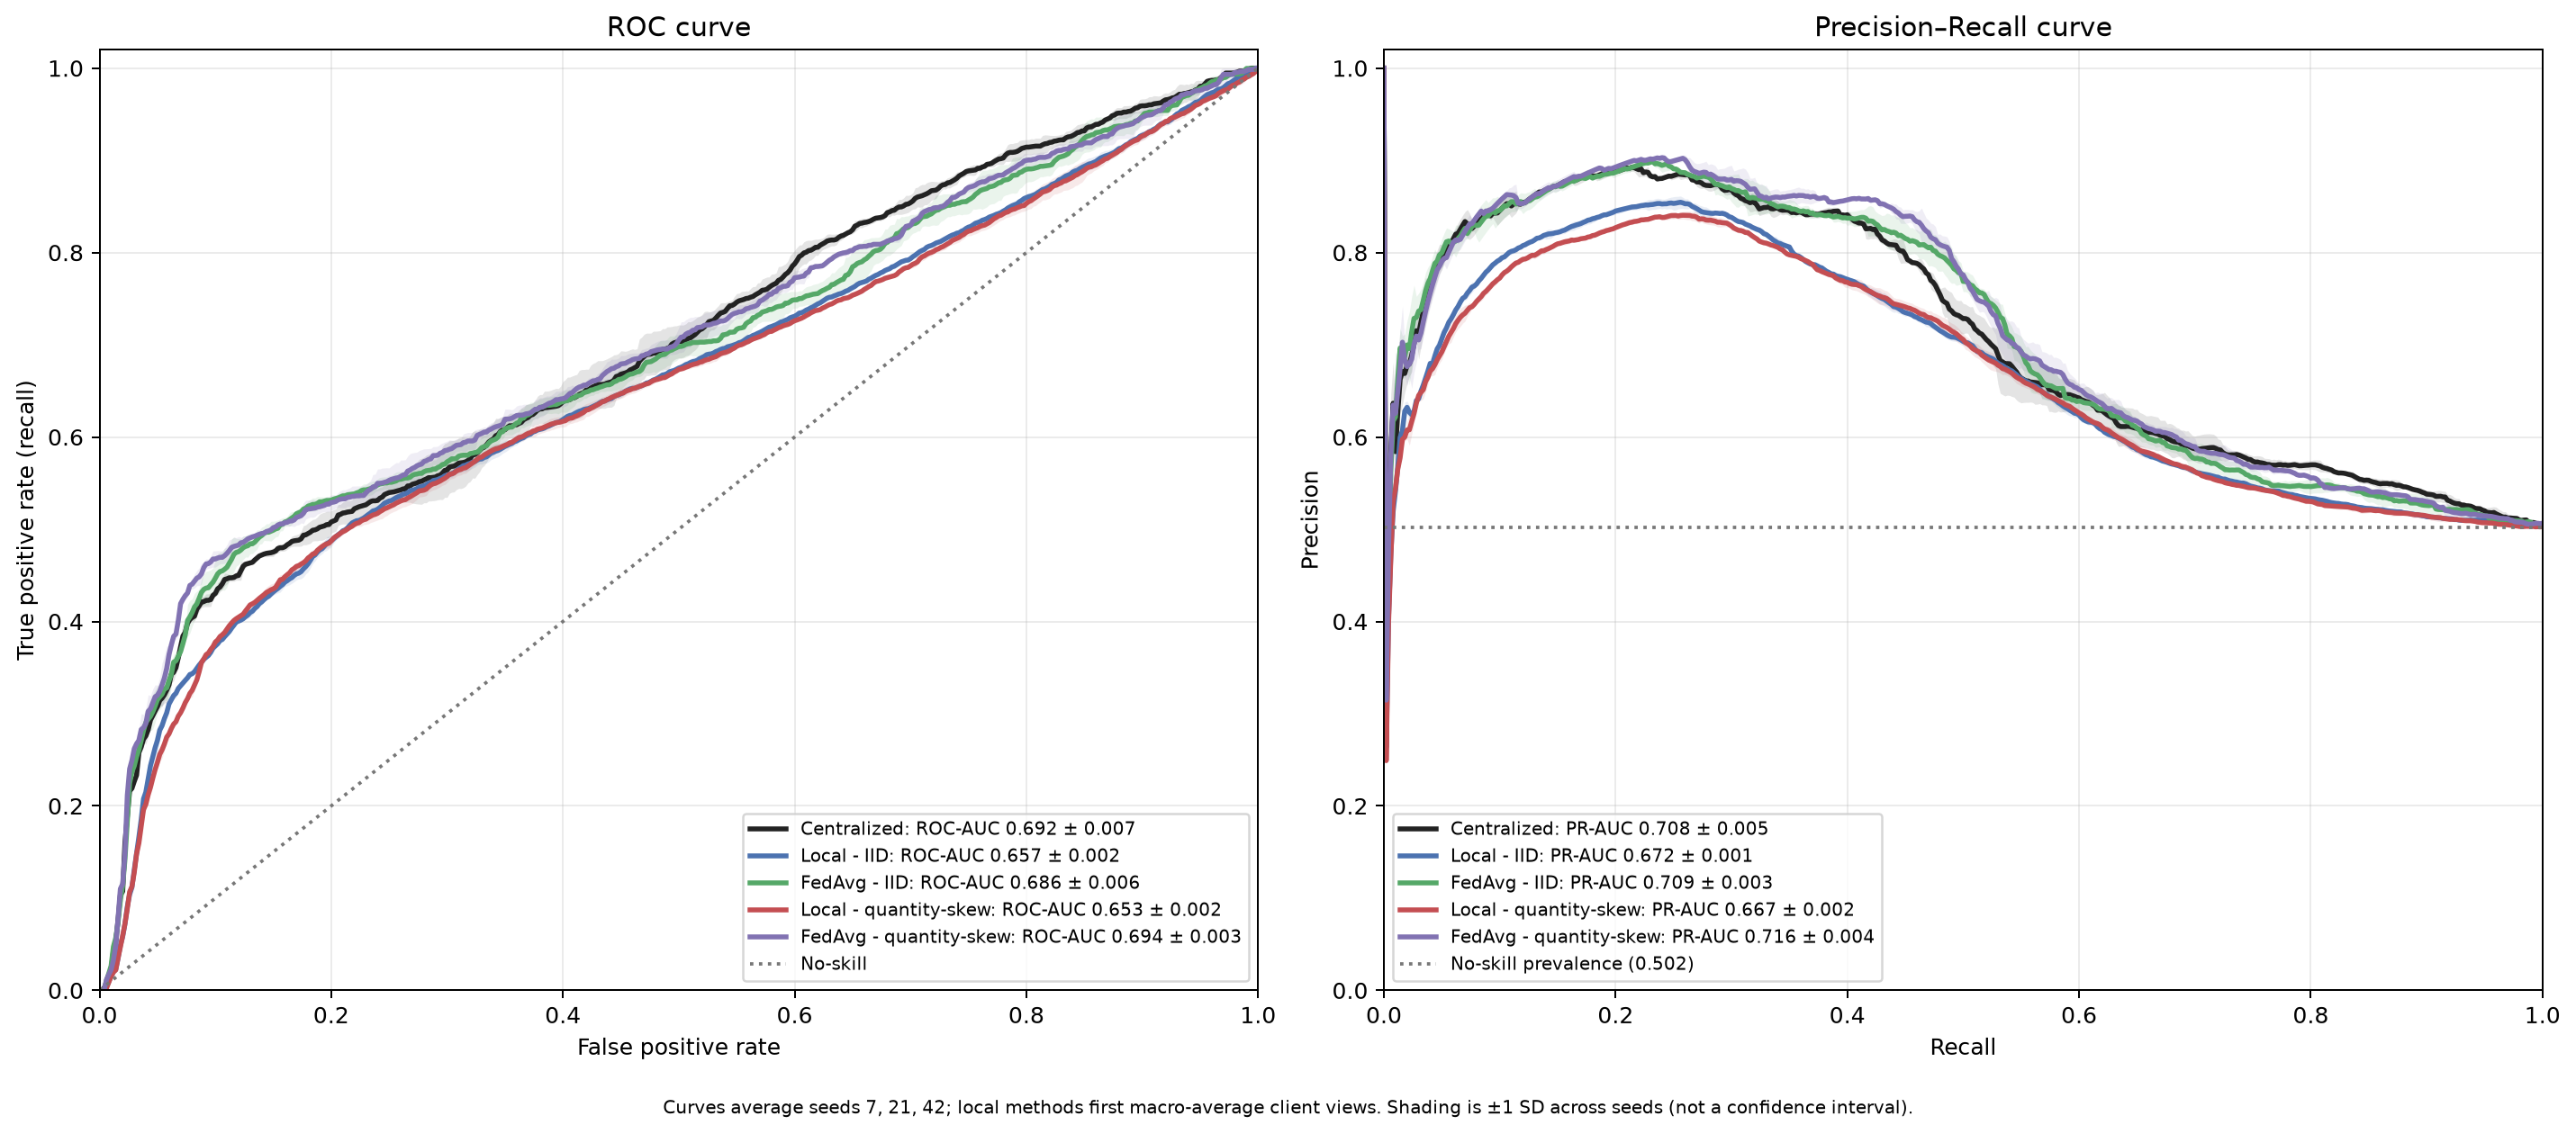
\includegraphics[width=\linewidth]{figures/roc_precision_recall_test_sensor_only_seeds_7_21_42.png}
		\caption{Precision-Recall curves}
		\label{fig:global_pr}
	\end{subfigure}
	\caption{Global ROC and Precision-Recall curves for the evaluated models, computed using the complete test set.}
	\label{fig:global_curves}
\end{figure*}

\textbf{Per-Client Performance}

Finally, the threshold-independent performance was examined at the client level to investigate variations in anomaly detection across the local test cohorts. Figure~\ref{fig:per_client_performance} presents the AP and ROC-AUC values for each client under the evaluated federated configurations.

\begin{figure*}[t]
	\centering
	\begin{subfigure}[b]{0.48\textwidth}
		\centering
		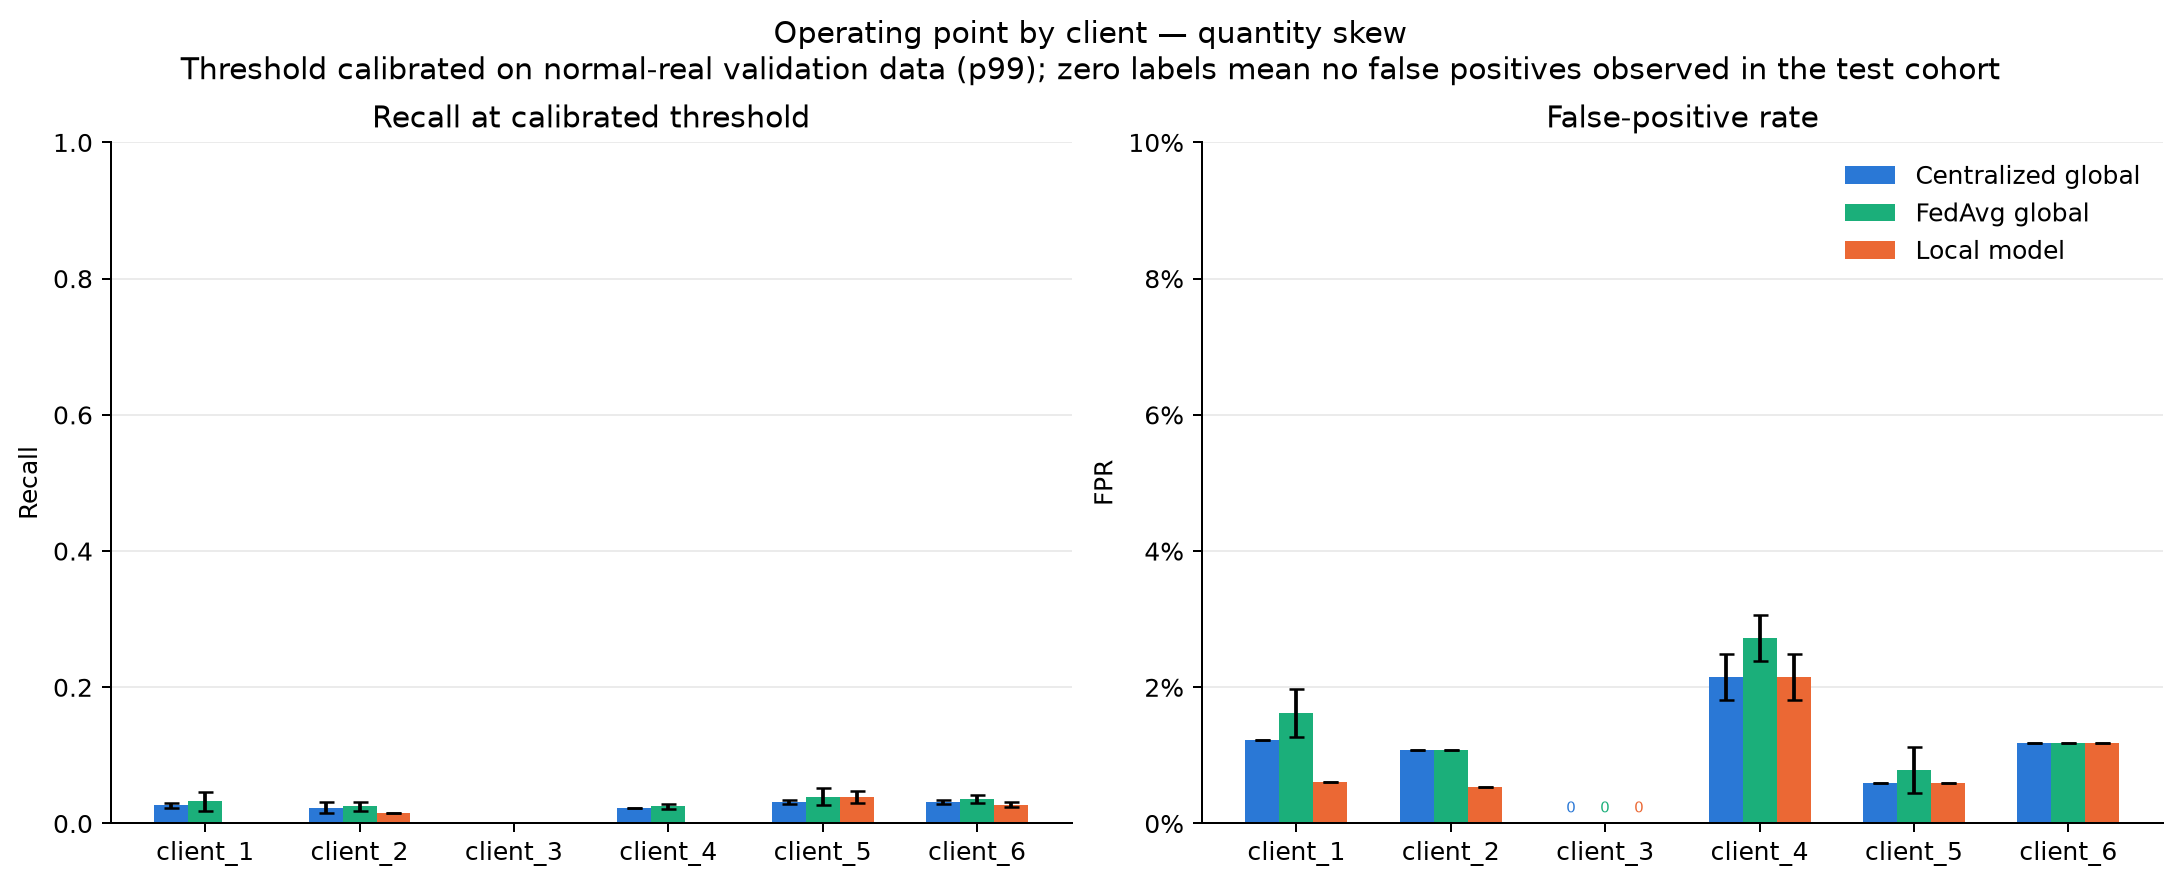
\includegraphics[width=\linewidth]{figures/client_test_operating_point_non_iid.png}
		\caption{Average Precision}
		\label{fig:per_client_ap}
	\end{subfigure}
	\hfill
	\begin{subfigure}[b]{0.48\textwidth}
		\centering
		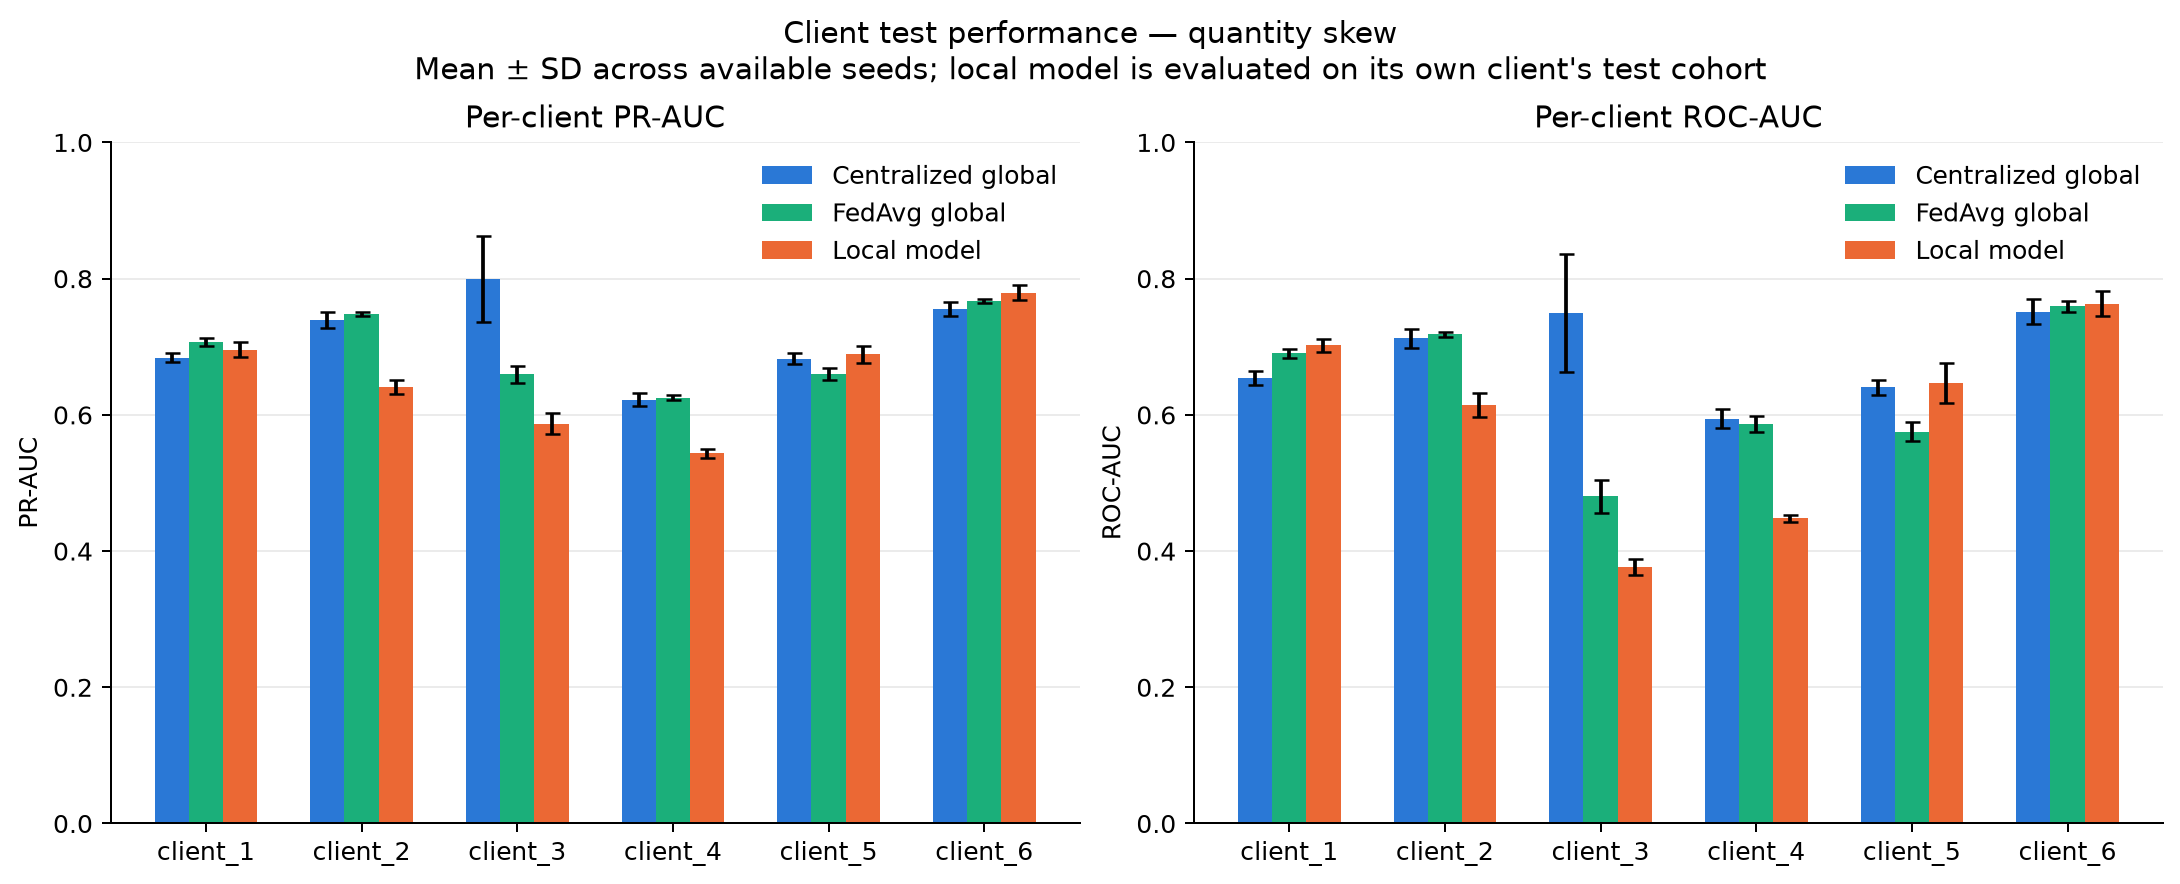
\includegraphics[width=\linewidth]{figures/client_test_auc_non_iid.png}
		\caption{ROC-AUC}
		\label{fig:per_client_roc_auc}
	\end{subfigure}
	\caption{Client-level threshold-independent anomaly detection performance.}
	\label{fig:per_client_performance}
\end{figure*}


\subsection{Raspberry Pi Detection results}

\begin{table*}[h!]
	\centering
	\caption{Anomaly detection performance for different local data volumes assigned to the Raspberry Pi client.}
	\label{tab:raspberry_volume_detection}
\centering
\resizebox{\columnwidth}{!}{%
	\begin{tabular}{|r|l|c|c|c|c|c|c|}
		\hline
		\textbf{Samples}          & \textbf{Method}     & \textbf{Accuracy}          & \textbf{Precision}         & \textbf{Recall}            & \textbf{F1-score}          & \textbf{PR-AUC}            & \textbf{ROC-AUC}           \\ \hline
		\multicolumn{1}{|c|}{380} & FedAvg              & \multicolumn{1}{r|}{0.587} & \multicolumn{1}{r|}{0.945} & \multicolumn{1}{r|}{0.184} & \multicolumn{1}{r|}{0.308} & \multicolumn{1}{r|}{0.704} & \multicolumn{1}{r|}{0.633} \\ \hline
		\multicolumn{1}{|c|}{318} & FedProx ($\mu=0.1$) & \multicolumn{1}{r|}{0.657} & \multicolumn{1}{r|}{0.903} & \multicolumn{1}{r|}{0.352} & \multicolumn{1}{r|}{0.506} & \multicolumn{1}{r|}{0.648} & \multicolumn{1}{r|}{0.496} \\ \hline
		\multirow{2}{*}{–}        & FedAvg              & –                          & –                          & –                          & –                          & –                          & –                          \\ \cline{2-8} 
		& FedProx ($\mu=0.1$) & –                          & –                          & –                          & –                          & –                          & –                          \\ \hline
		\multirow{2}{*}{–}        & FedAvg              & –                          & –                          & –                          & –                          & –                          & –                          \\ \cline{2-8} 
		& FedProx ($\mu=0.1$) & –                          & –                          & –                          & –                          & –                          & –                          \\ \hline
	\end{tabular}%
}
\end{table*}

\subsection{Raspberry Pi Computational Performance}

\begin{table*}[h!]
	\centering
	\caption{Computational and communication performance of the Raspberry Pi client under different local data volumes.}
	\label{tab:raspberry_computational}
	\small
	\begin{tabular}{llrcccccc}
		\toprule
		\textbf{Scenario} &
		\textbf{Method} &
		\textbf{Local samples} &
		\textbf{Training time (s)} &
		\textbf{Time/epoch (s)} &
		\textbf{Throughput (samples/s)} &
		\textbf{CPU (\%)} &
		\textbf{Peak RAM (MB)} &
		\textbf{Temperature ($^\circ$C)} \\
		\midrule
		\multirow{2}{*}{Low}
		& FedAvg              & -- & -- & -- & -- & -- & -- & -- \\
		& FedProx ($\mu=0.1$) & -- & -- & -- & -- & -- & -- & -- \\
		\midrule
		\multirow{2}{*}{Medium}
		& FedAvg              & -- & -- & -- & -- & -- & -- & -- \\
		& FedProx ($\mu=0.1$) & -- & -- & -- & -- & -- & -- & -- \\
		\midrule
		\multirow{2}{*}{High}
		& FedAvg              & -- & -- & -- & -- & -- & -- & -- \\
		& FedProx ($\mu=0.1$) & -- & -- & -- & -- & -- & -- & -- \\
		\bottomrule
	\end{tabular}
\end{table*}

\subsection{Discussion}
 

\section{Conclusion}


\section{References}

\bibliographystyle{sbc}
\bibliography{sbc-template}

\end{document}
